\scanpage{40}
On obtient ainsi
\[
(10)\qquad f(t)=\frac1{3\sqrt{-3}}\frac{(t+1)(2t-1)(t-2)}{t(t-1)}
\]
et par suite
\[
\boxed{\begin{array}{c|c}\unsure{g^*(t)|f^*g^*(t)}=(gf)^*(t)&j=\dfrac1{-27}\left(\dfrac{(t+1)(2t-1)(t-2)}{t(t-1)}\right)^2\end{array}}\qquad(11)
\]
Cette formule, comme il se doit, est définie sur $S$ lui-même, et non seulement sur $S'$ ! Elle définit un revêtement galoisien de groupe $\mathfrak S_3$ de \deleted{$\unsure{(G_a)_S}$} $P^1_S$, \inserted{\unsure{à partir de} $(G_a)_S$,} qui est non ramifié au dessus de $(G_{\unsure{m|a}})_S-(0)-(1)=(G_m)_S-1$.
\figure{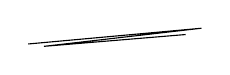
\begin{tikzpicture}\draw (0,0)--(2.2,.2)--(.2,-.03)--(2,.12);\end{tikzpicture}}

Comment opère $\sigma$ dans les quotients ?
\margin{\diagram{\begin{tikzcd}[row sep=large]
\sigma\quad P^1\arrow[d,"f"]\\
\sigma'\quad P^1\arrow[d,"g"]\\
\sigma''\quad P^1
\end{tikzcd}}}
On voit que $\sigma'(\infty)=0$, $\sigma'(0)=\infty$, $\sigma'(1)=1$, d'où mêmes formules pour $\sigma''$, d'où
\[
\deleted{\sigma'(t)=1/t}
\]
\deleted{et d'autre part}
\[
(11)\qquad\sigma'(t)=\sigma''(t)=1/t
\]
et il \unsure{serait} facile de \unsure{prouver} ces équations \unsure{pour $\sigma$ dans ce dernier cas} (p.ex.).
\figure{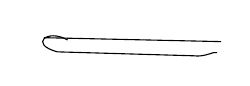
\begin{tikzpicture}\draw (0,.1) .. controls (-.25,.25) and (-.5,.05) .. (-.13,-.05)--(1.6,-.1) .. controls (1.75,-.12) and (1.85,-.04) .. (1.9,-.06);\draw (-.3,.13)--(1.95,.08);\end{tikzpicture}}
\mspage{39}
